\documentclass[11pt, a4paper, english]{NTNUoving}
\usepackage[utf8]{inputenc}
\usepackage[T1]{fontenc}
\usepackage{float}
\usepackage{enumitem}
\usepackage{csquotes}
\usepackage{listings}
\usepackage{listings}
\usepackage{color}
\usepackage{biblatex}
\usepackage{mathtools}
\usepackage{hyperref}
\ovingnr{5}    % Nummer på innlevering
\semester{Spring 2021}
\fag{Optimization and Control \\ TTK4135}
\institutt{Department for Engineering Cybernetics}

\begin{document}

%1
\begin{oppgave}

    %a
    \begin{punkt}
        \begin{align*}
            A &= \begin{bmatrix}
                0 & 0 & 0 \\
                0 & 0 & 1 \\
                0.1 & -0.79 & 1.78
            \end{bmatrix} \\
            \implies \det(A-\lambda I) &= 0 \\
            \implies -\lambda(-\lambda(1.78-\lambda) + 0.79) &= 0 \\
            \implies \lambda_1 = 0.844 \wedge \lambda_2 &= 0.936
        \end{align*}
        Since $|\lambda_i| \leq 1$ for $i \in \{1,2\}$ the system is stable.
    \end{punkt}

    %b
    \begin{punkt}
        $n_x = 3$ since $x_t$ is a vector multiplied by A which is a $3 \times 3$ matrix.

        $n_u = 1$ since $u_t$ is a vector multiplied by B which is a $3 \times 1$ matrix.

        $Q$ and $R$ is defined as:

        \begin{align*}
            Q &= 2\begin{bmatrix}
                C & 0 \\
                0 & 0
            \end{bmatrix}
            = 2 \begin{bmatrix}
                0 & 0 & 0 \\
                0 & 0 & 0 \\
                0 & 0 & 2
            \end{bmatrix} \\
            R &= 2r = 2
        \end{align*}

        The multiplication by 2 comes because the objective function is divided by 2 in the formulation.

    \end{punkt}

    %c
    \begin{punkt}

        Since $Q$ is positive semidefinite and $R$ is positive definitive this is a convex QP problem. The convexity
        depends on $Q$, $R$ and $C$ (because $Q$ depends on $C$).

    \end{punkt}

    %d
    \begin{punkt}
        \label{1d}

        The state space model is:
        \begin{align*}
            x_{t+1} &= Ax_t + Bu_t \\
            \implies x_1 -Ax_0 -Bu_0 &= 0 \Leftrightarrow Ix_1 - Ax_0 - Bu_0 = 0 \\
             x_2 -Ax_1 -Bu_1 &= 0 \Leftrightarrow Ix_2 - Ax_1 - Bu_1 = 0 \\
            &\shortvdotswithin{=}
             x_N -Ax_{N-1} -Bu_{N-1} &= 0 \Leftrightarrow Ix_{N} - Ax_{N-1} - Bu_{N-1} = 0
        \end{align*}

        With $z = \begin{bmatrix}
            x_1^\top, x_2^\top, ..., x_N^\top, u_0^\top, u_1^\top, ..., u_{N-1}^\top
        \end{bmatrix}$ and moving $Ax_0$ to the other side of the equation since $x_0$ isn't in $z$:

        \begin{align*}
            b_{eq} &= \begin{bmatrix}
                Ax_0 \\
                0 \\
                \vdots \\
                0
            \end{bmatrix} \\
            A_{eq} &= \begin{bmatrix}
                I & 0 & \dots &  \dots & 0 & -B & 0 & \dots & \dots & 0 \\
                -A & I & \ddots &  & \vdots & 0 & \ddots & \ddots & & \vdots \\
                0 & -A & \ddots & \ddots & \vdots & 0 & \ddots & \ddots & \ddots & \vdots \\
                \vdots &  & \ddots & \ddots & 0 & \vdots &  & \ddots & \ddots & 0 \\
                0 & \dots & 0 & -A & I & 0 & \dots & \dots & 0 & -B
            \end{bmatrix}
        \end{align*}

        The KKT system is then (from the book):
        \begin{align*}
            \begin{bmatrix}
                G &  -A^\top_{eq} \\
                A_{eq} & 0
            \end{bmatrix} \begin{bmatrix}
                z^\star \\
                \lambda^\star
            \end{bmatrix} = \begin{bmatrix}
                0 \\
                beq
            \end{bmatrix}
        \end{align*}
        \begin{figure}[H]
            \centering
            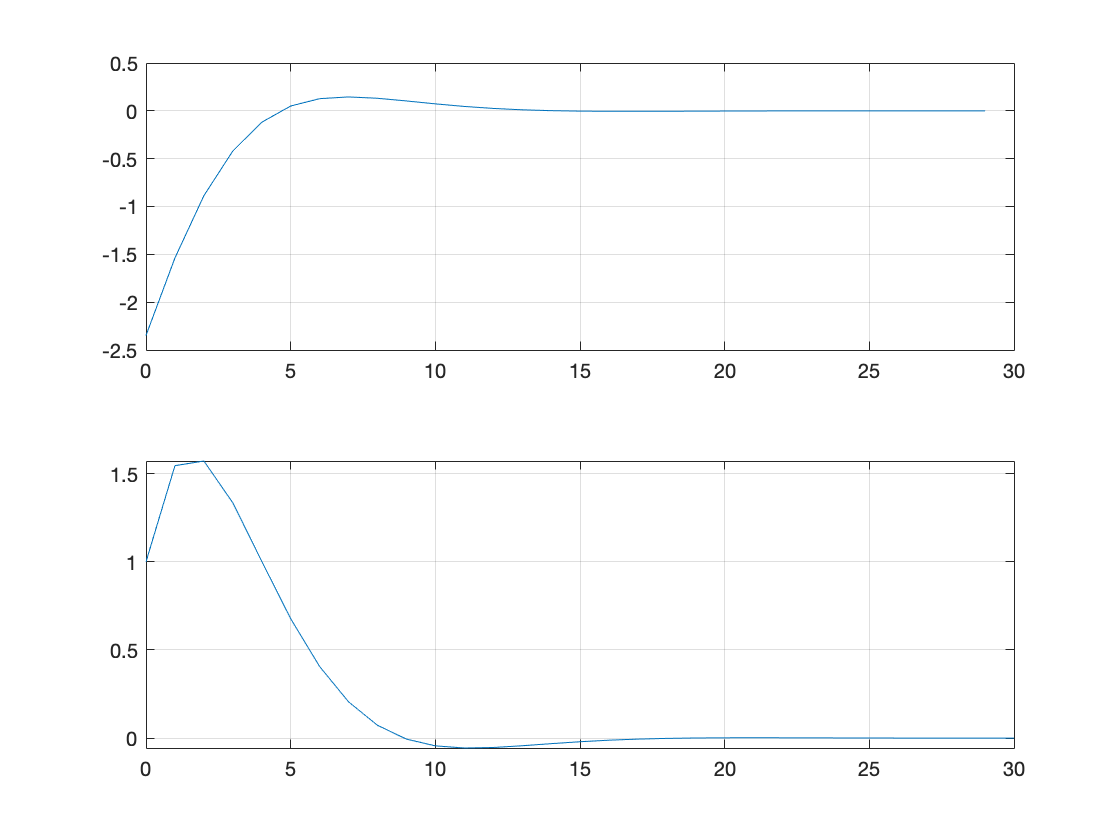
\includegraphics[width=0.8\textwidth]{../1d.png}
            \caption{Solution by solving the KKT conditions.}
            \label{fig:1e1}
        \end{figure}


    \end{punkt}

    %e
    \begin{punkt}

        The plots in Figure \ref{fig:1e1}, \ref{fig:1e2} and \ref{fig:1e3} shows the results with the \texttt{quadprog} function with different
        values of $r$. As we can see the solution is the same as in Task \ref{1d} when $r=1$.
        When we make $r$ smaller we see that the control inputs are steeper, this is because we allow for larger values of $u_i$
        in the objective function, when we make $r$ larger the control inputs are smoother since larger control inputs are punished more.

        \begin{figure}[H]
            \centering
            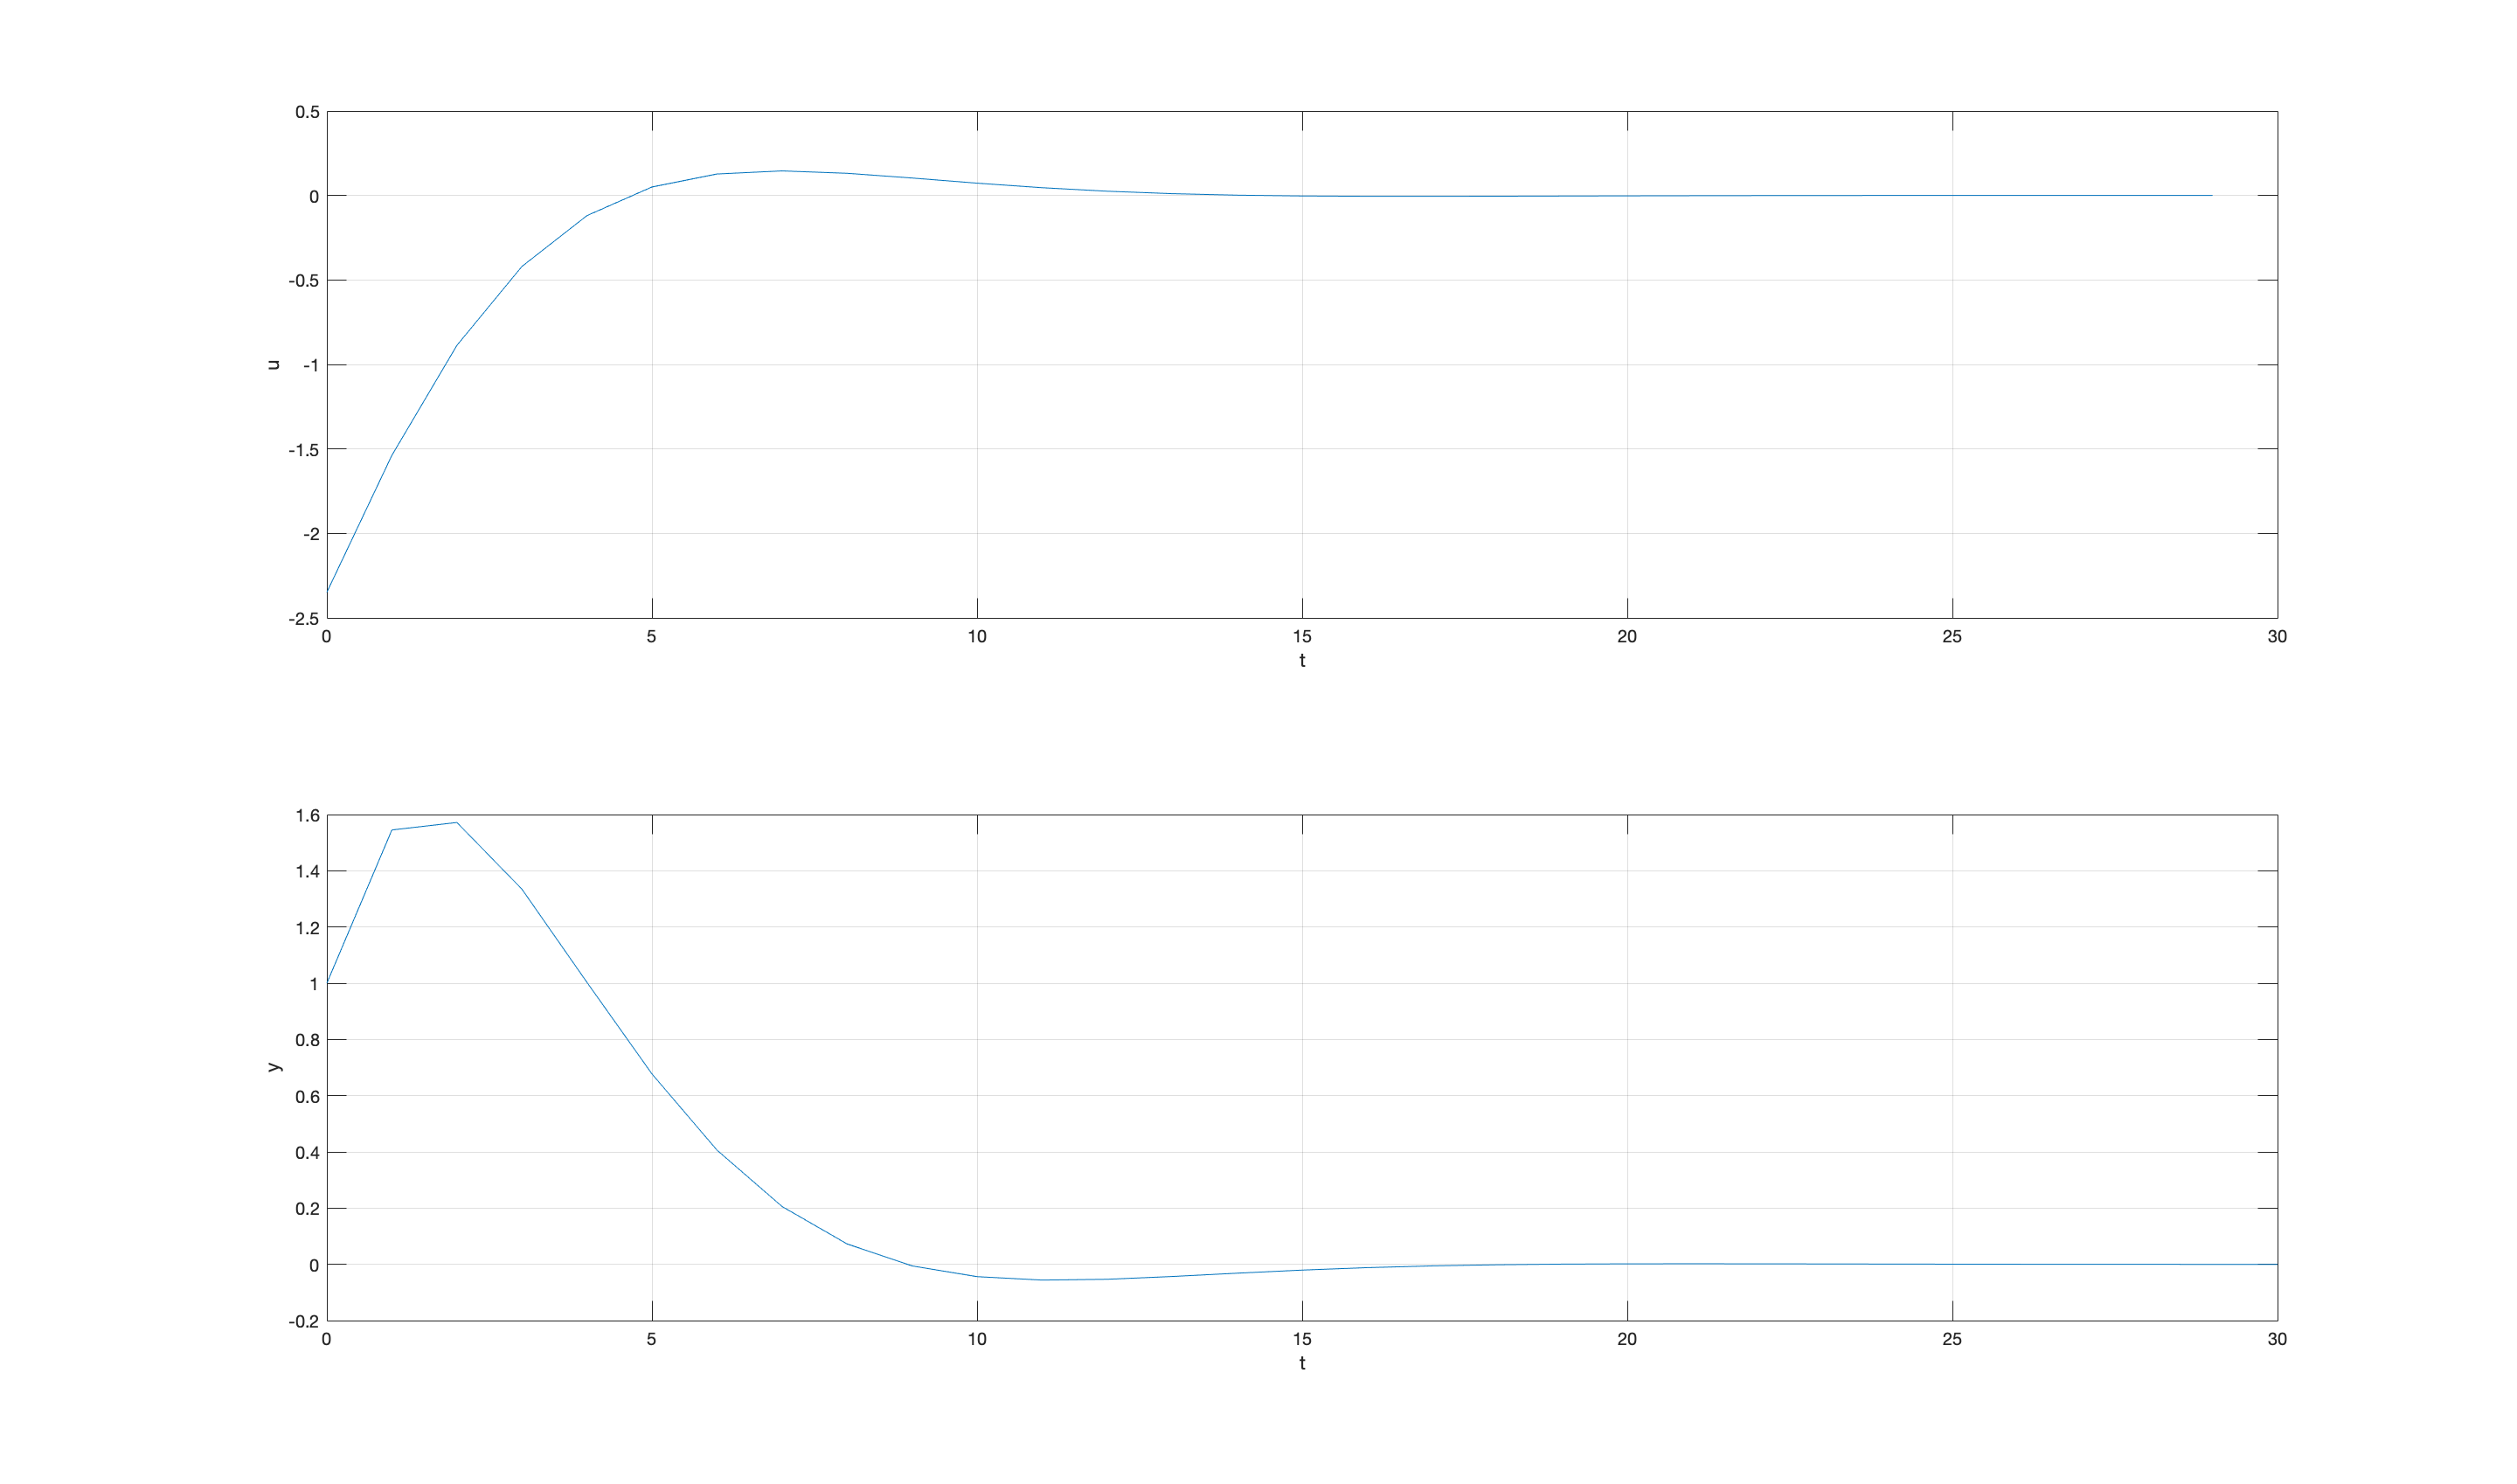
\includegraphics[width=0.8\textwidth]{../1e_rd.png}
            \caption{$u_t$ and $y_t$ with $r=1$.}
            \label{fig:1e1}
        \end{figure}


        \begin{figure}[H]
            \centering
            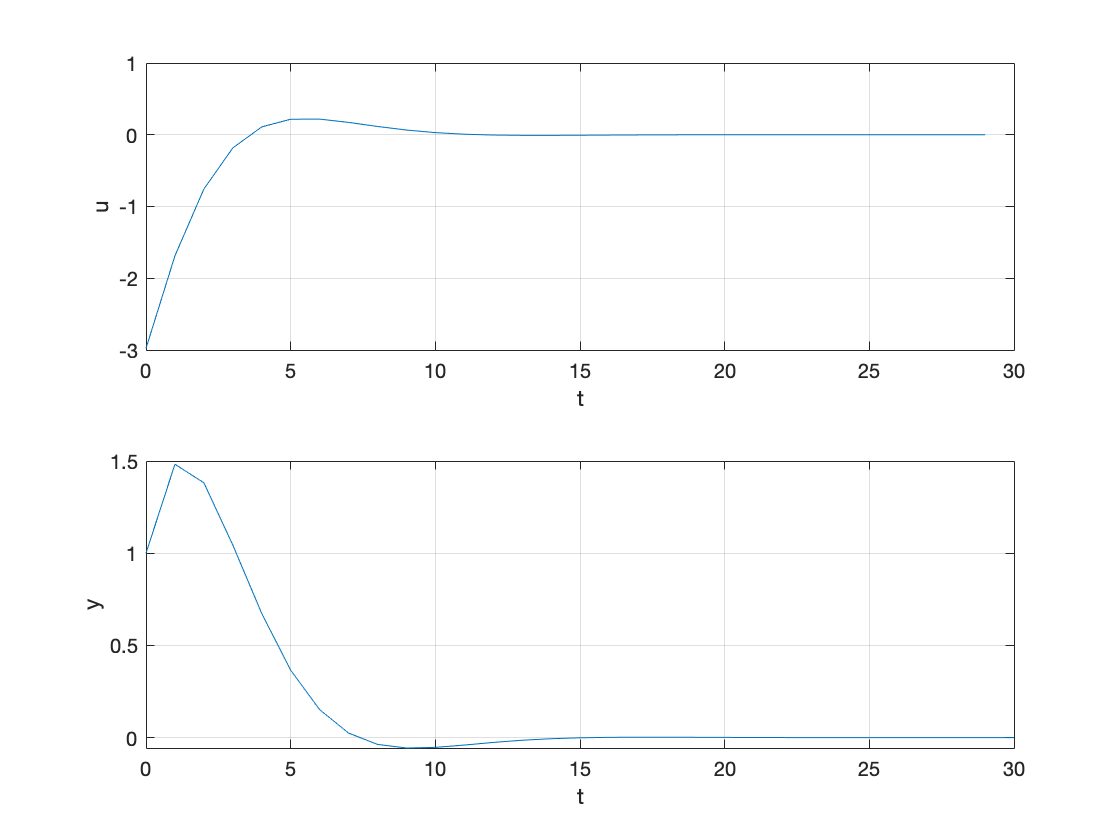
\includegraphics[width=0.8\textwidth]{../1e_r1.png}
            \caption{$u_t$ and $y_t$ with $r=0.5$.}
            \label{fig:1e2}
        \end{figure}

        \begin{figure}[H]
            \centering
            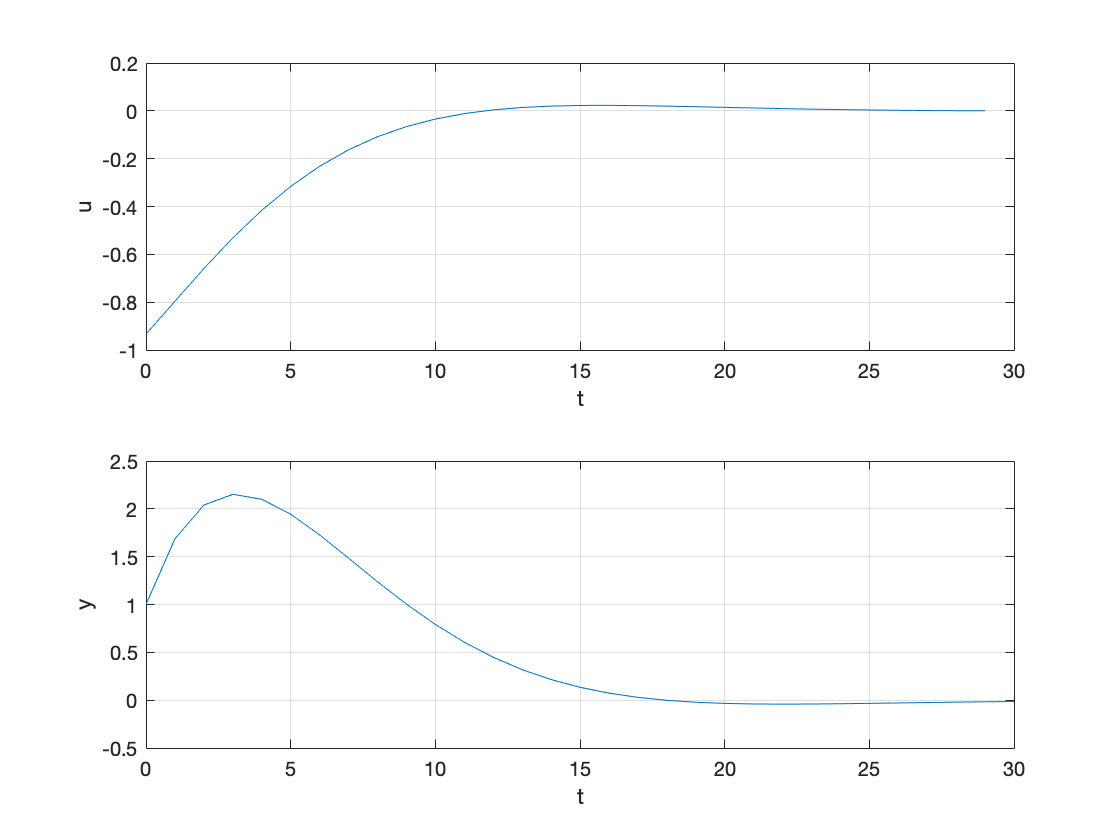
\includegraphics[width=0.8\textwidth]{../1e_r2.png}
            \caption{$u_t$ and $y_t$ with $r=10$.}
            \label{fig:1e3}
        \end{figure}


    \end{punkt}

    %f
    \begin{punkt}
        \label{1f}
        The resulting plot is in Figure \ref{fig:1f}. The number of iterations with \texttt{quadprog} was 5, this increase comes because the QP is
        now inequality constrained, which is harder to solve.
        \begin{figure}[H]
            \centering
            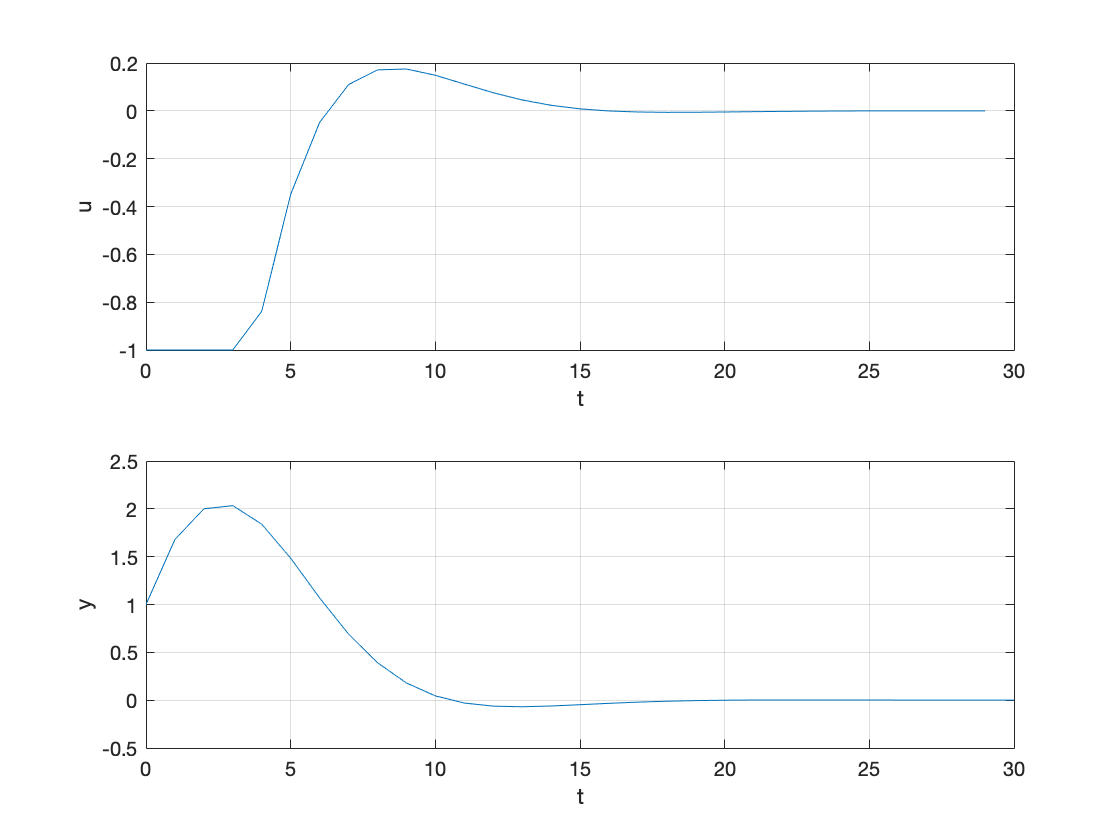
\includegraphics[width=0.8\textwidth]{../1f.png}
            \caption{$u_t$ and $y_t$ for inequality constrained control input.}
            \label{fig:1f}
        \end{figure}
    \end{punkt}

\end{oppgave}

%2
\begin{oppgave}

\begin{punkt}
Model predictive control is a regulation method for finding the optimal inputs of control at an instant. MPC does this by using finite-horizon open-loop control at a certain sampling.
The main advantage of MPC is that it will keep the future in mind when optimizing (thus "predictive"). Since MPC is open-loop it doesn't directly involve feedback, but MPC works by sampling at a certain rate and is thus able to
include feedback at every sampling step.

\begin{figure}[H]
    \centering
    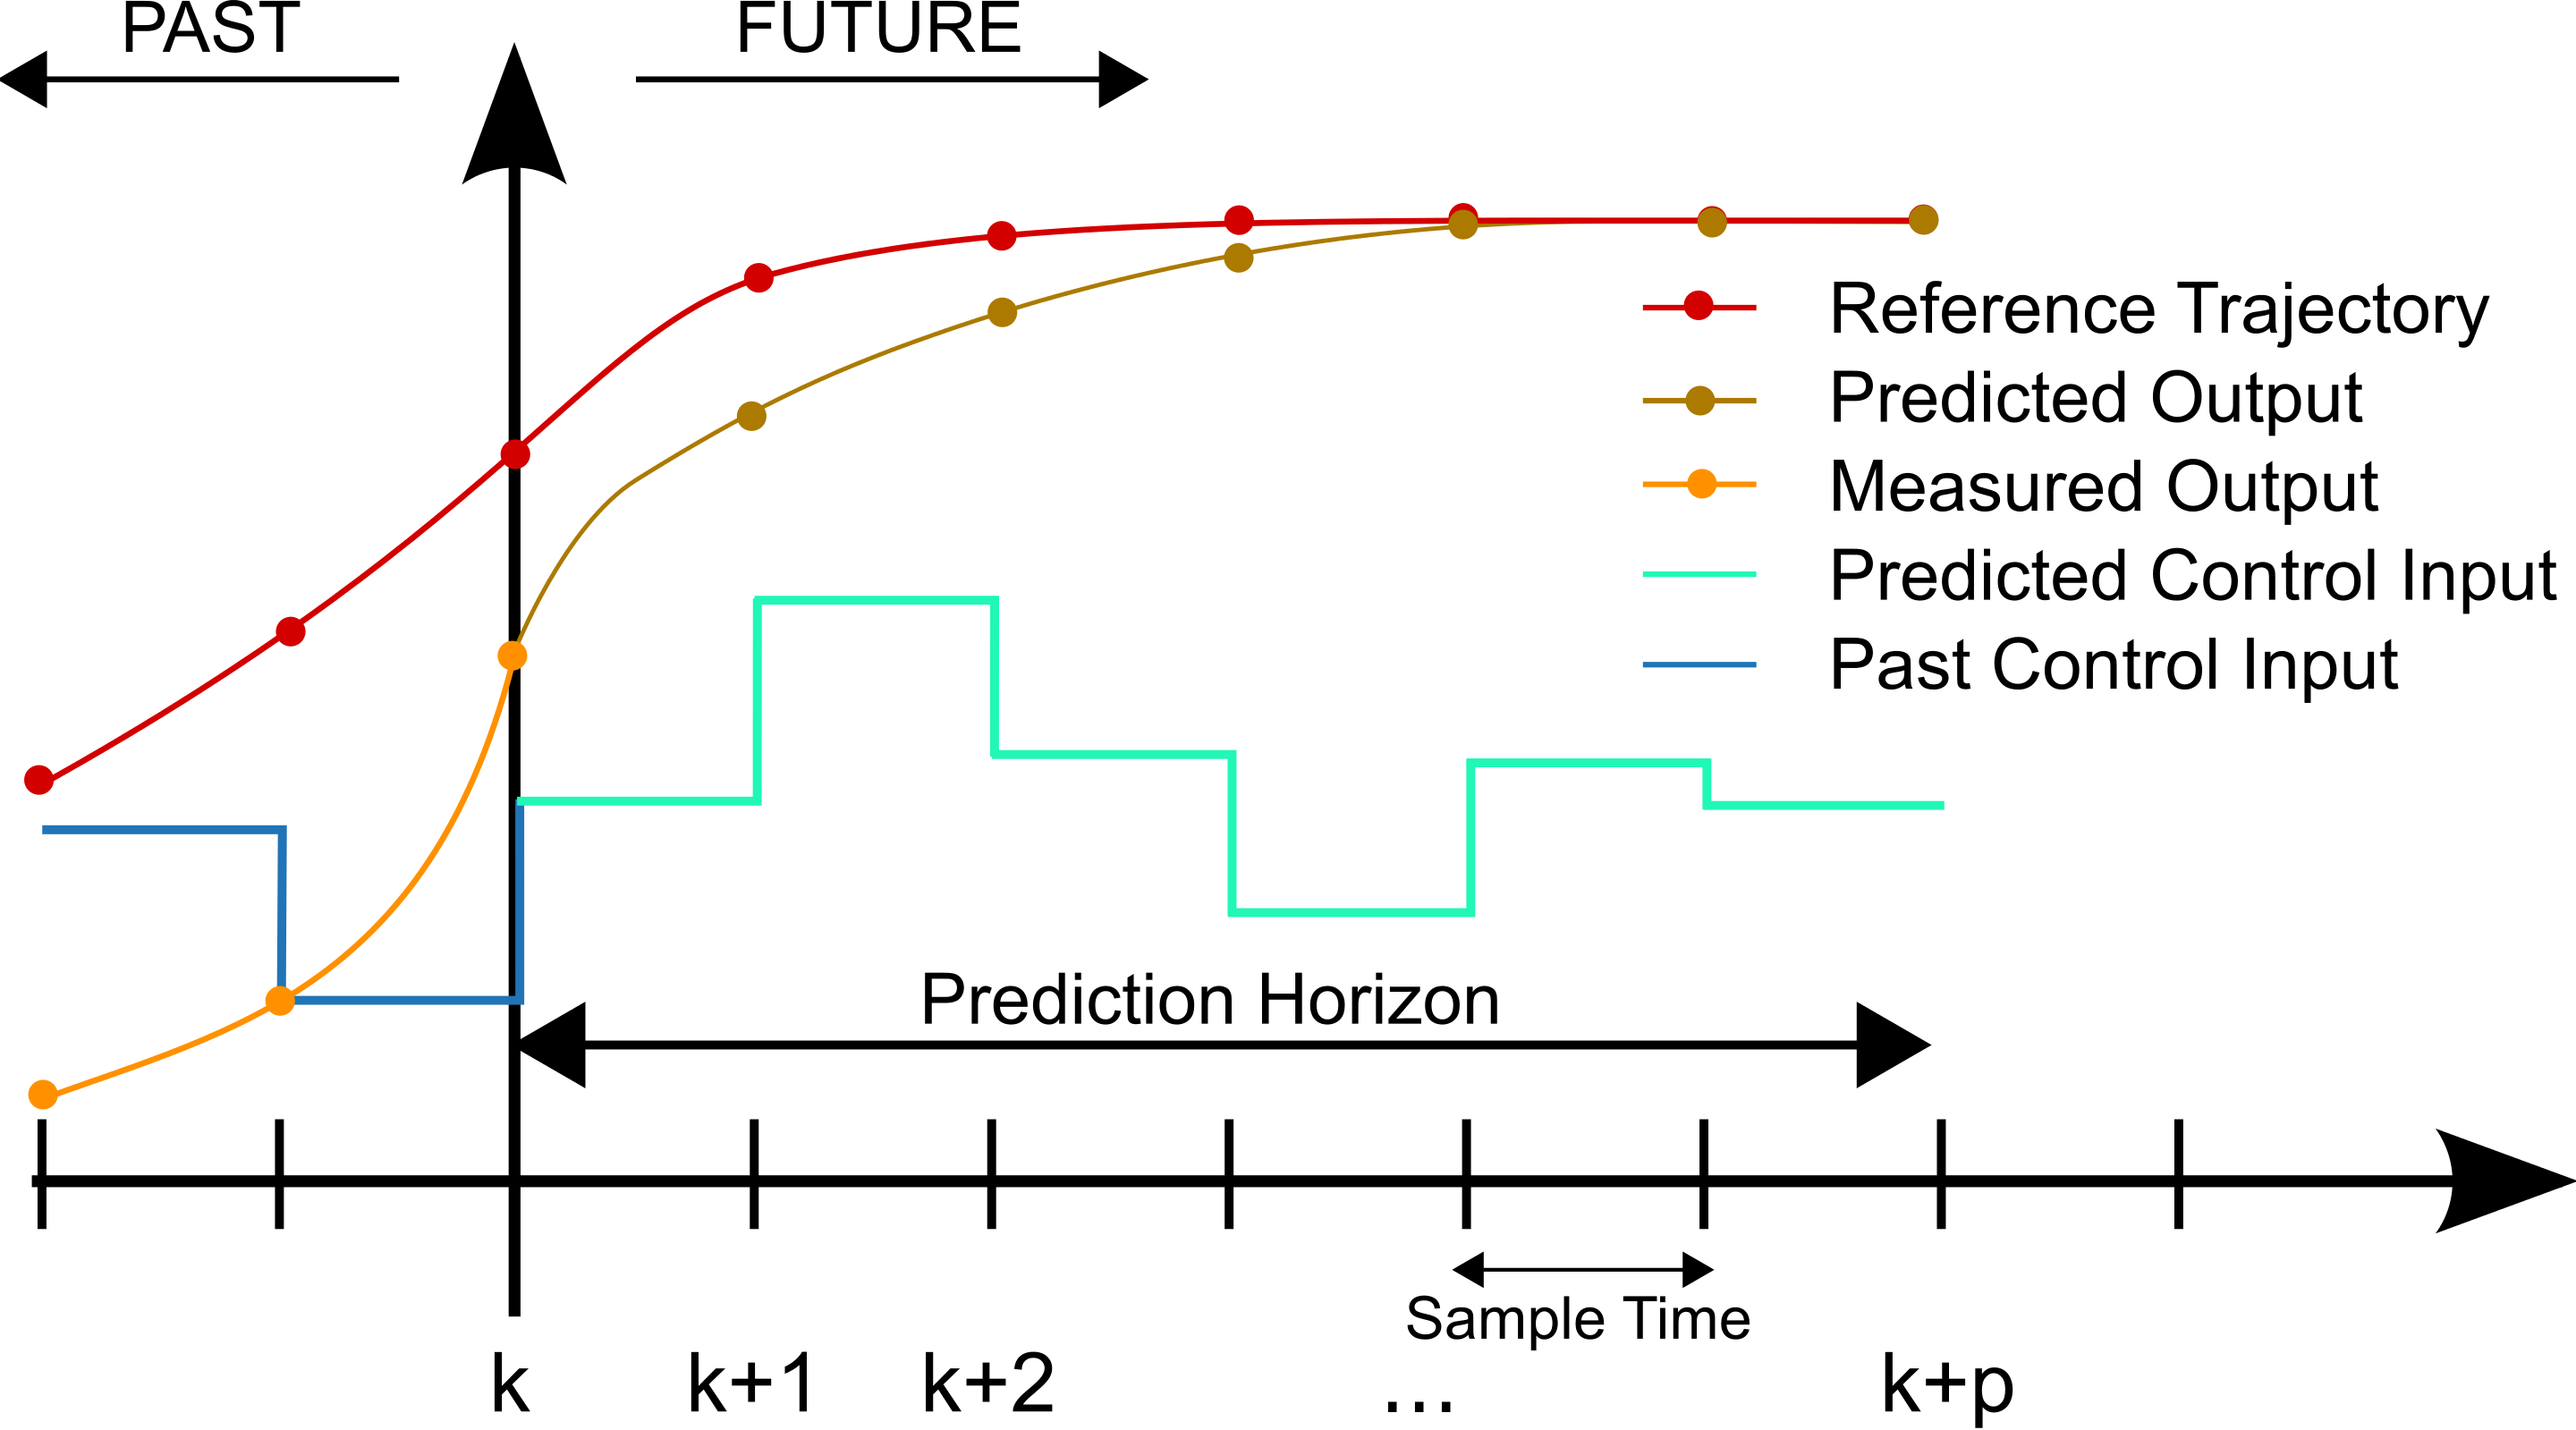
\includegraphics[width=0.8\textwidth]{MPC_scheme_basic.png}
    \caption{This figure shows how the MPC will optimize over a finite-horizon timeline and predicting the outcome of the control inputs to achieve an optimal sequence of inputs.}
\end{figure}


\end{punkt}

\begin{punkt}
    The resulting plot is found in Figure \ref{fig:2b}. As we can see this solution is very similar to our open-loop prediction over the whole horizon in Task \ref{1f}.
    \begin{figure}[H]
        \centering
        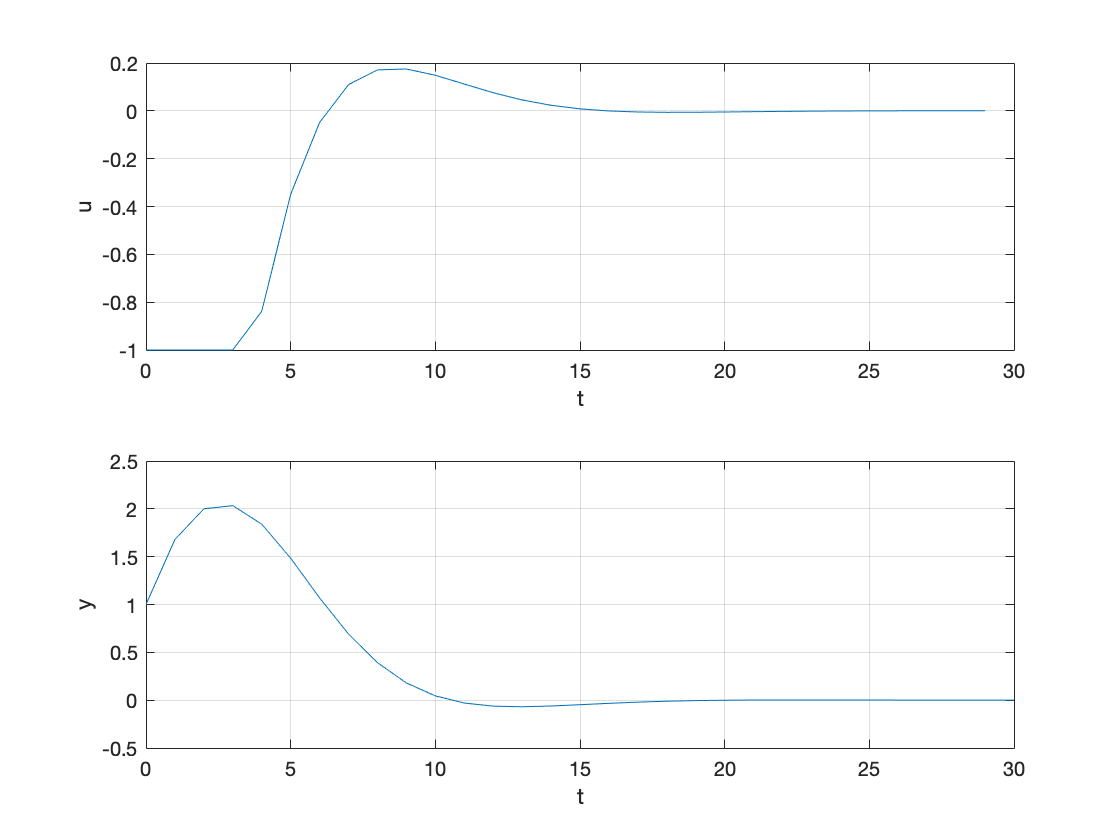
\includegraphics[width=0.8\textwidth]{../2b.png}
        \caption{$u_t$ and $y_t$ for MPC with horizon of 30.}
        \label{fig:2b}
    \end{figure}
\end{punkt}

\begin{punkt}
    The resulting plot is found in Figure \ref{fig:2c}. As we can see the MPC must use more input into the system and it doesn't get the $y_t$ to zero before $t=30$, this
    happens because the differences between the model in MPC and the real plant makes the MPC's control inputs non-optimal for the real plant.
    \begin{figure}[H]
        \centering
        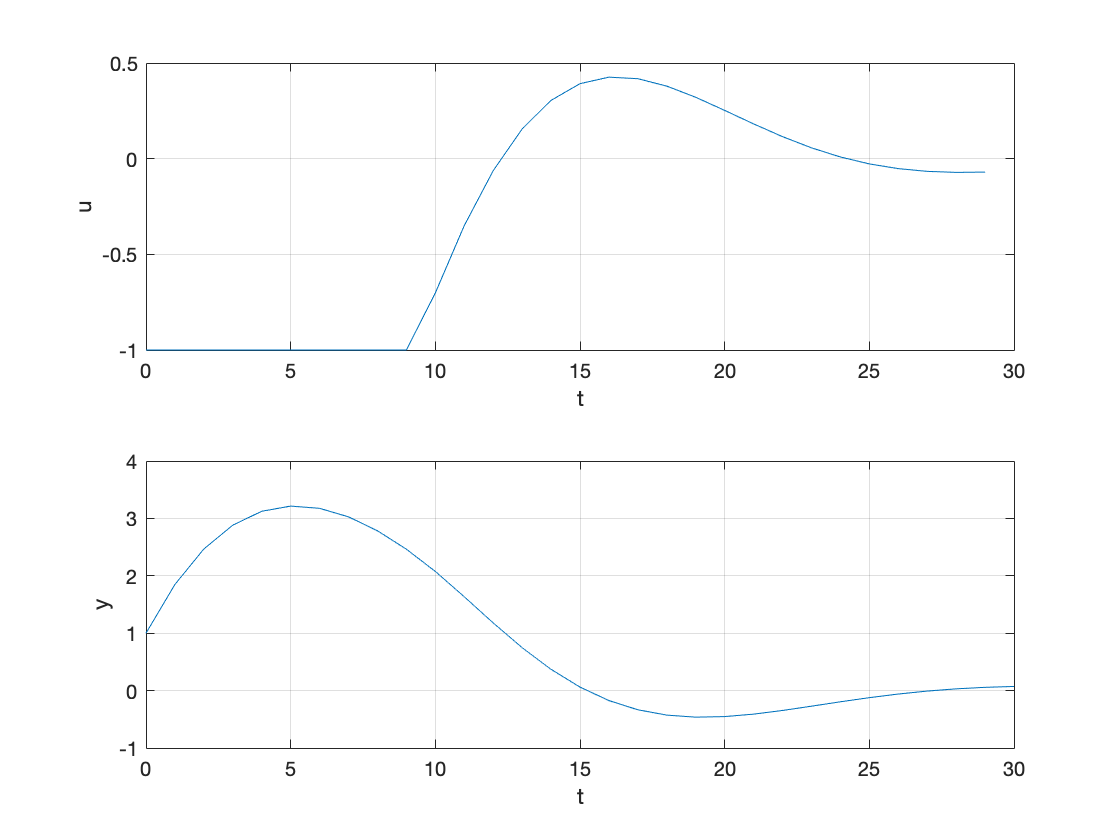
\includegraphics[width=0.8\textwidth]{../2c.png}
        \caption{$u_t$ and $y_t$ for MPC with horizon of 30 and different plant between MPC model and simulation.}
        \label{fig:2c}
    \end{figure}
\end{punkt}
\end{oppgave}

\end{document}
